\chapter{Polymorphic malwares and Sandboxes}

\section{Polymorphic malwares and viruses}

Even if attackers are lazy,
they react to countermeasures,
and in fact have developed mechanisms to hide (obscure) information
in the program to prevent a positive match against signatures.

\subsection{Encryption}
A tecnique is to encrypt malware and viruses.
Upon infection, each copy of the virus program creates a
new version by generating a new key and by encrypting the
body of the virus.
Sometimes the decryptor code is prepended to the actual malware, 
but even if not, it must exist somewhere and it can be
detected.

\begin{figure}[htbp]
   \centering
   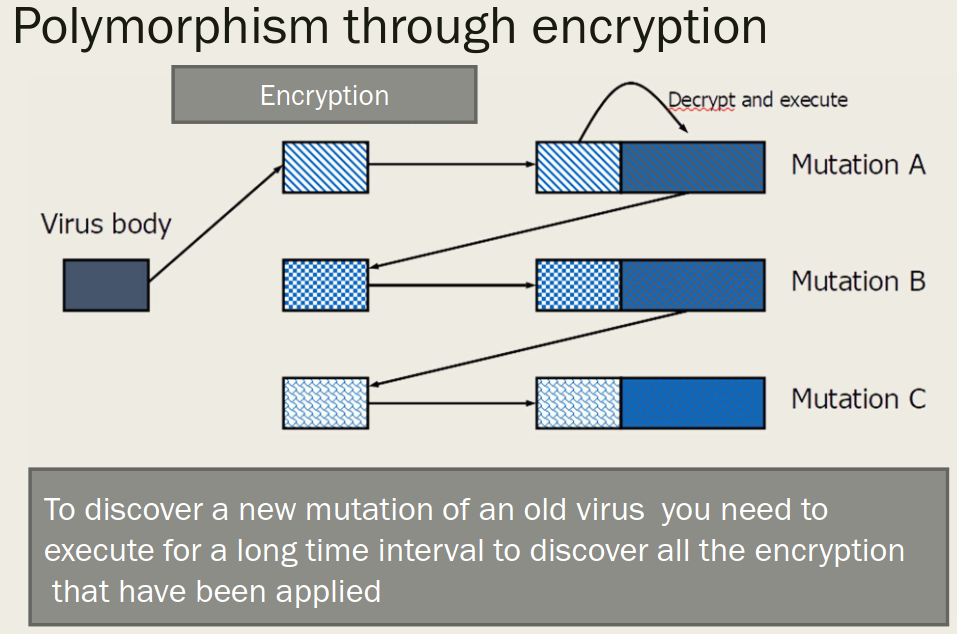
\includegraphics{images/polymorphism_encryption.png}
   \caption{Polymorphism through encryption}
   \label{fig:polymorphism_encryption}
\end{figure}

\subsection{\texttt{Emotet} example}
\begin{figure}[htbp]
   \centering
   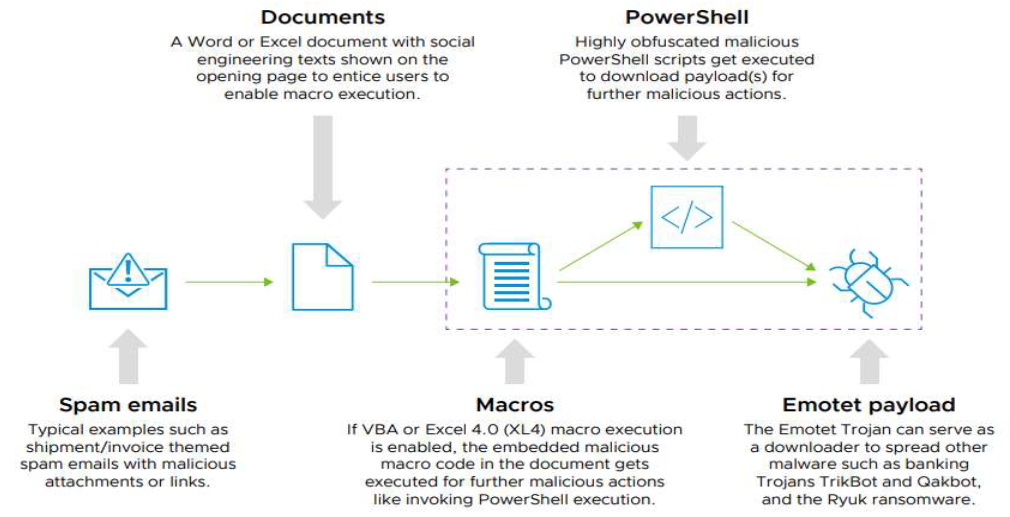
\includegraphics{images/emotet.png}
   \caption{Emotet}
   \label{fig:emotet}
\end{figure}

A new Emotet wave was observed in late January 2022.13 that introduced
the use of the \texttt{mshta.exe} application to carry out the infection,
which is a legal Windows-native utility which \textit{Microsoft HTML Application}
(\texttt{HTA}) files "fooled" into performing malicious actions\footnote{This kind of attack is known as \textit{confused deputy attack}}.\nl

HTA files are basically HTM with enhanced privileges. 
When encoding, HTA
allows the developer to have the features of HTML together with the
advantages of scripting languages that sometimes are not present for html-based.

Emotet provided malicious HTA files containing highly obfuscated JScript code.
On a dataset with 19,791 samples with non-trivial execution chains, 139 unique program chains and 20,955 unique invocation chains were identified.

\subsection{\texttt{Zmist} example}

Designed in 2001 by the russian virus writer \texttt{Z0mbie}
The virus fragments are interleaved with fragments of the host application and are stored at random positions connected by memory jumps.
When and if the virus is executed, it will infect any executable. 
The starting point of the virus cannot be reached in some execution because it is randomly generated.


\section{Sandboxes}
Recall that a \textbf{sandbox} is a \textit{protected environment} to download and execute potentially risky code;
it is disjoint and confined from the normal execution environment and usually hosted
on a cloud.
It allows to analyze and test a code without
interaction with the system to be protected.
Ideally, in a sandbox the code can do anything but escaping and thus accessing resources of the real system.

A sandbox is nothing but a specific purpose, highly robust \textbf{virtual machine}
that detects anomalous behavior 
\note{(erasing/ encrypting files etc...)}

Sandboxes can be used both for defence and analysis.
They can be \textbf{riskful}, 
since if the malware escapes the sandbox then it may cause damage to the system.
Besides nowdays malwares can discover whether they are running in a VM and defeat the detection by behaving correctly in the VM.

\subsection{Detecting Sandboxes}
Most VMs require that the VM runs some software tools, called guest
additions which support file sharing between the host and the VM or even simple
copy and paste operations between applications on the host and the VM.
The presence of such  guest additions is one of the easiest and most direct things to
check to detect a VM.

To communicate from inside the VM to the host and vice versa, VMMs use
things like shared memory or special instruction sequences.
Even if the guest
additions are not installed, these mechanisms are there to make guest
additions work can be detected.

Besides, some malware look for signs of a system used by a normal user doing routine
things as opposed to a clean system for a special purpose, like analysing
malware.
Usually, malware analysis starts with a clean VM because it is simpler
to get a clean VM going for each malware analysis and having a clean system
removes a lot of variability

There is a debate on compatibility against transparency.